\chapter{Stuguinシステム}
本章では,学習に対する動機づけの内在化を目的としたシステム,Stuguinを提案する.
はじめにStuguinシステムの概要を述べ,次にStuguinの特徴を説明する.
そして最後に,ユーザがStuguinを利用する流れについて述べる.

\section{Stuguinシステムの概要}
Stuguinは学習記録を管理するアプリケーションである.
学習時間の測定ができ,教科・内容とともに記録することができる.
保存された学習記録は,その時間や内容ごとにグラフで可視化される.
また,ポイント機能,ランキング機能,目標設定機能が存在し,この内一つがトップ画面に表示される.

\section{Stuguinシステムの特徴}
本節では,Stuguinシステムの特徴としてあげられる機能を3つ挙げる.

\subsection{動機づけタイプに応じた機能の切り替え}
Stuguinは,ユーザの動機づけタイプに合わせて機能の切り替えが行われる.
ユーザが動機づけ測定アンケートに回答することで,結果に応じてトップ画面に表示される機能が変更されるものである.
表示される機能は,ポイント,ランキング,目標設定の内いずれか一つである.
これにより,ユーザが抱く動機づけに沿ったアプローチを行うことができると考える.

\subsection{学習記録の可視化}
Stuguinは,ユーザの学習記録を棒グラフや円グラフで可視化する.
この機能では過去の学習記録の時間や教科,内容,記録の頻度などを閲覧が可能である.
これにより,ユーザは達成感を感じたり,学習の偏りに気づいたりすることができる.

\subsection{スマートフォン利用の制限}
Stuguinでは,学習時間を計測する際,スマートフォンの利用を制限する.
正確には,学習時間の計測中にStuguinが閉じられた場合,学習が中断され他のアプリケーションが利用されているものとみなし,直ちに記録を終了する.
デバイス自体がロックされた場合はこの限りではないため,ユーザはスマートフォンから離れて学習に集中することができる.

\section{Stuguinシステムの使用方法}
本アプリケーションを開くと,図~\ref{fig:top}のようなトップ画面が開かれる.

ユーザはまず,トップ画面下にある``Study"ボタンより,学習を記録する.
記録には,実際に測定する方法と手動で入力する方法の2種類がある.
実際に測定する方法を選択した場合には,ストップウォッチのようにして学習時間を測定する.
測定中の画面を図~\ref{fig:measure4}に示す.

1件でも学習記録が保存されると,図~\ref{fig:outline4}のようにトップ画面に学習記録の概要が表示されるようになる.
ユーザは日ごとや週ごとの学習時間を棒グラフで,学習した教科や内容の割合を円グラフで閲覧することができる.
また,学習を記録した日が色付けされたカレンダーも生成される.

週に一度,動機づけに関するアンケートがユーザに対して実施される.
アンケート回答画面を~\ref{fig:questionnaire4}に示す.
このアンケートによりユーザの動機づけタイプが測定され,その結果に応じてトップ画面に表示される機能が切り替わる.
ポイント機能では学習時間に応じた獲得ポイントが,ランキング機能は他ユーザも合わせた総学習時間のランキングが表示される.
目標設定機能の場合は,はじめにユーザはその週の目標学習時間を設定するよう指示される.
以後は目標に対する達成割合が表示される.

\begin{figure}[ht]
\begin{center}
\begin{tabular}{c}

	\begin{minipage}[b]{0.5\linewidth}
	\begin{center}
		\fbox{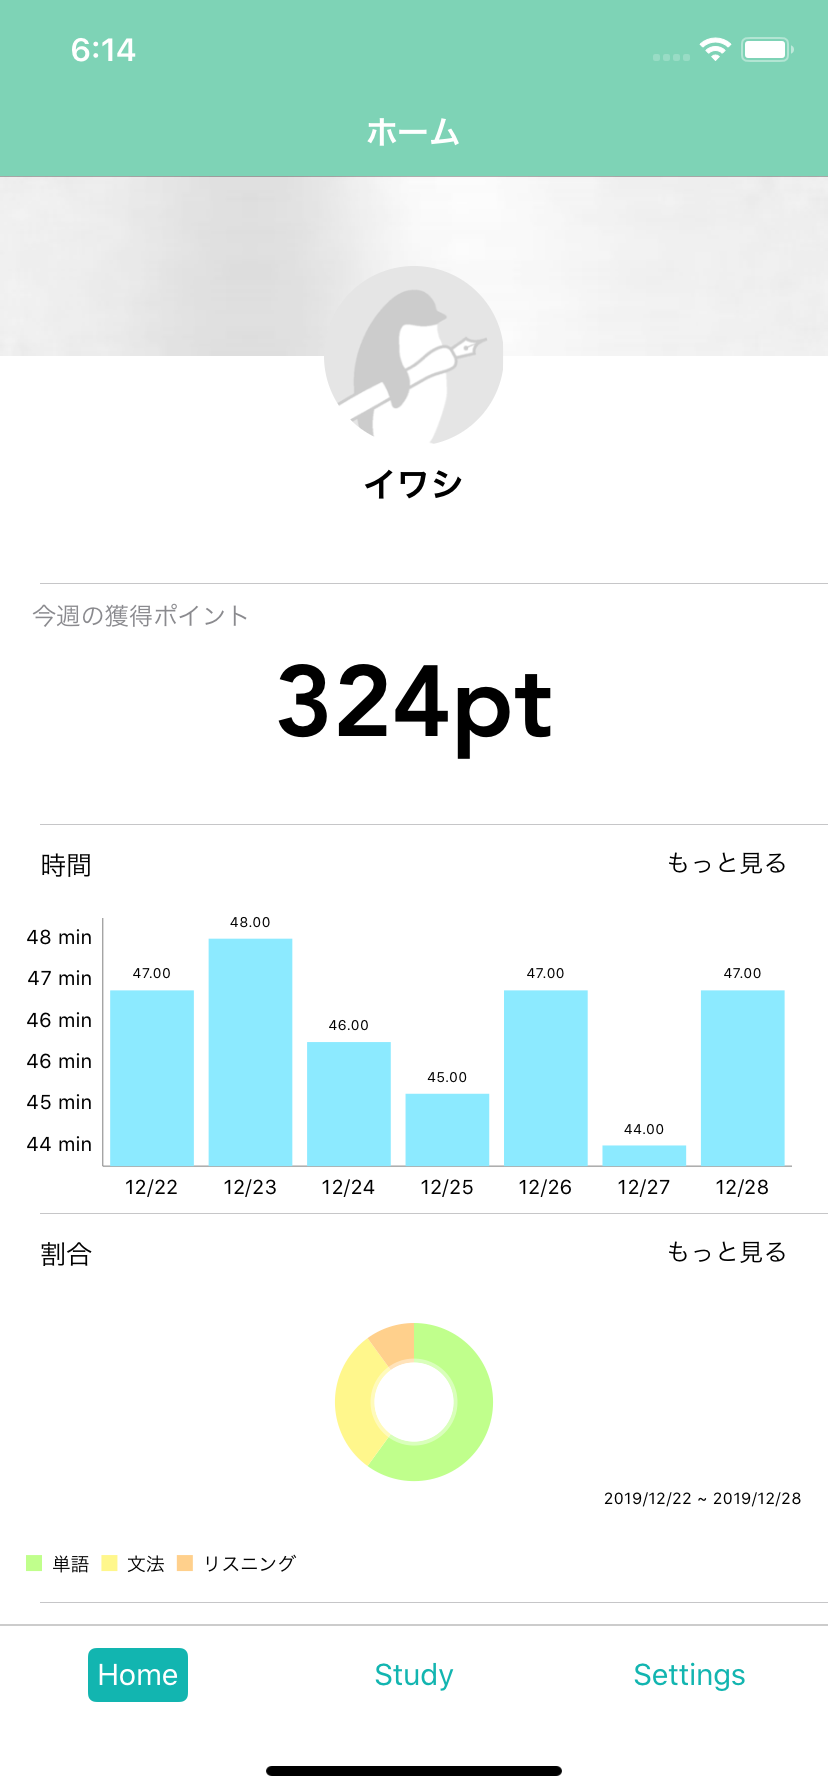
\includegraphics[width=5cm]{images/4/top.png}}
		\caption{Stuguinシステムのトップ画面}
		\label{fig:top}
	\end{center}
	\end{minipage}

	\begin{minipage}[b]{0.5\linewidth}
	\begin{center}
		\fbox{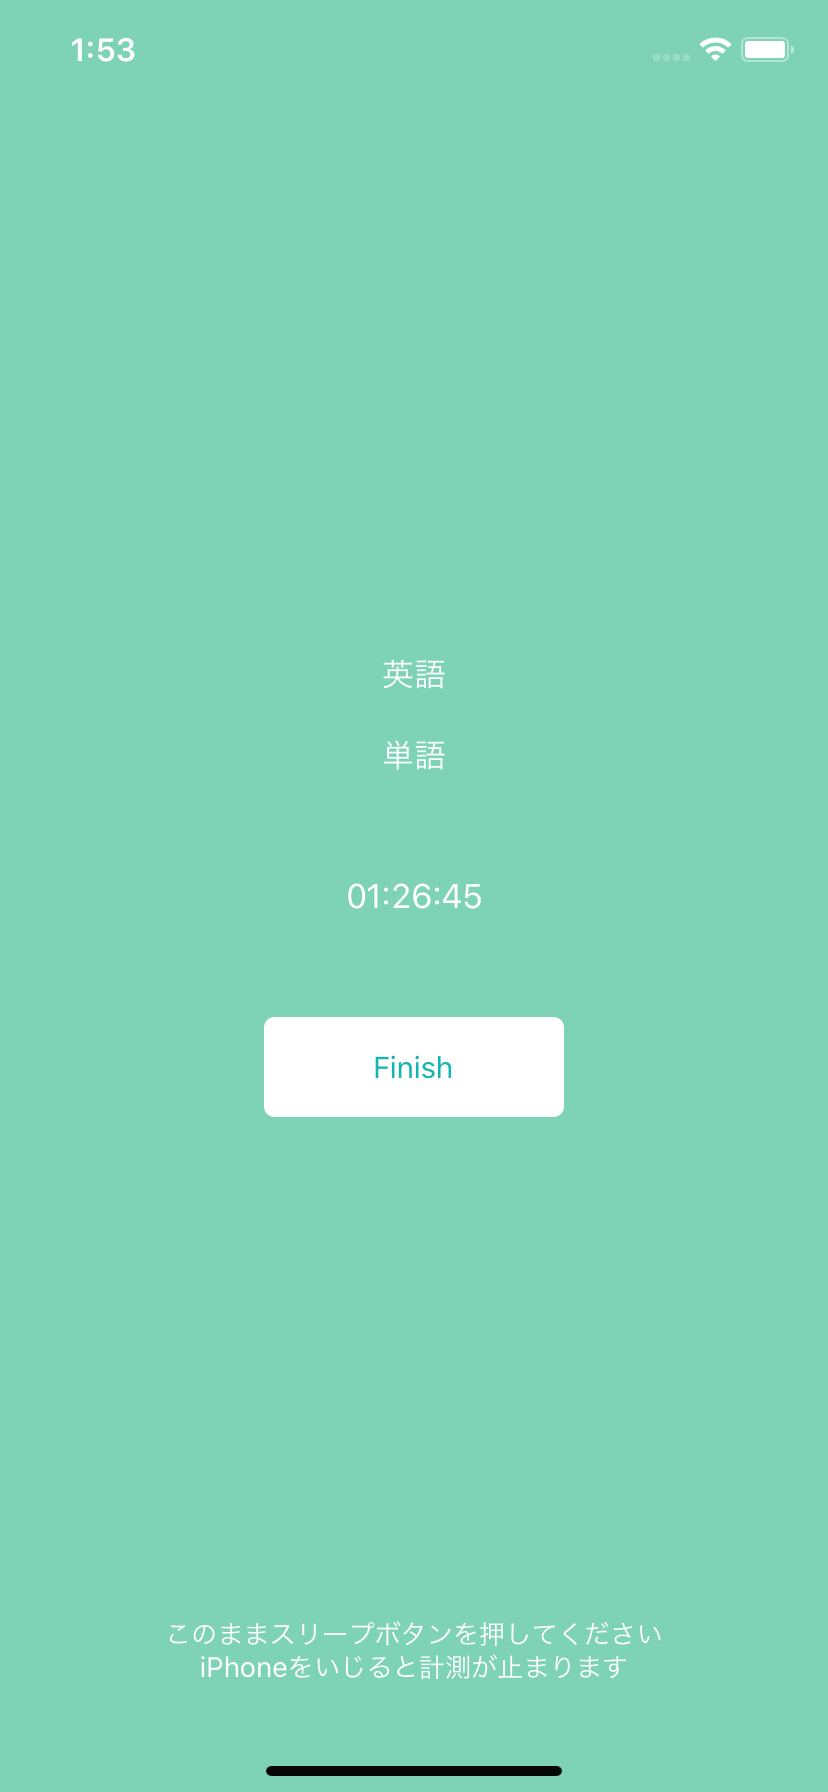
\includegraphics[width=5cm]{images/4/measure.png}}
		\caption{学習時間測定画面}
		\label{fig:measure4}
	\end{center}
	\end{minipage}

	\\

	\begin{minipage}[b]{0.5\linewidth}
	\begin{center}
		\fbox{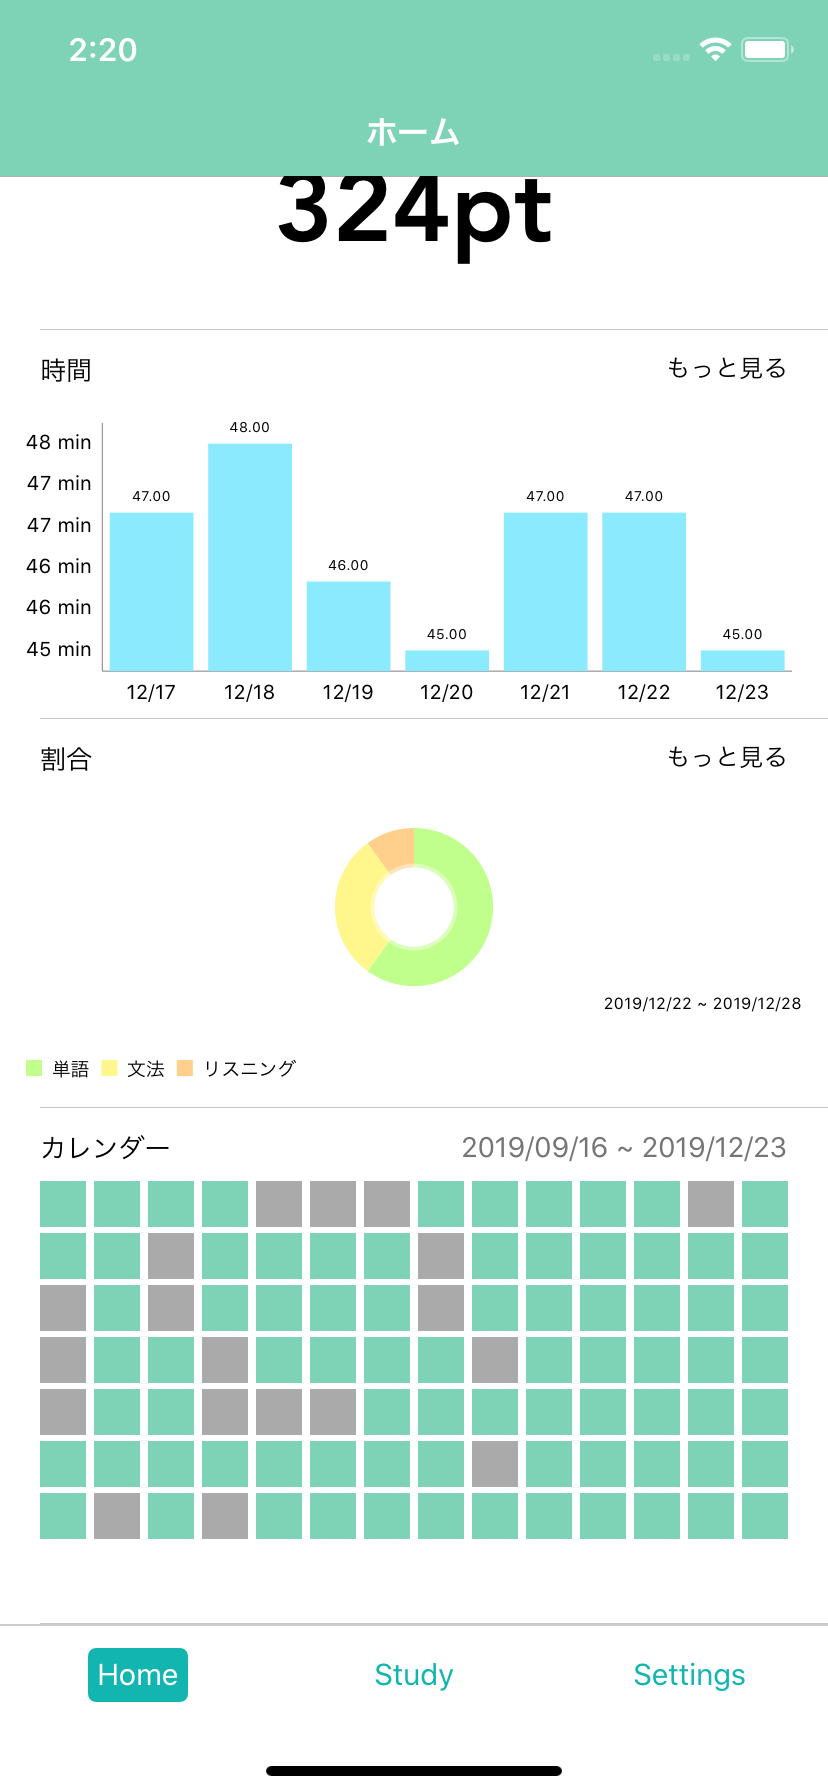
\includegraphics[width=5cm]{images/4/outline.png}}
		\caption{学習記録の概要}
		\label{fig:outline4}
	\end{center}
	\end{minipage}

	\begin{minipage}[b]{0.5\linewidth}
	\begin{center}
		\fbox{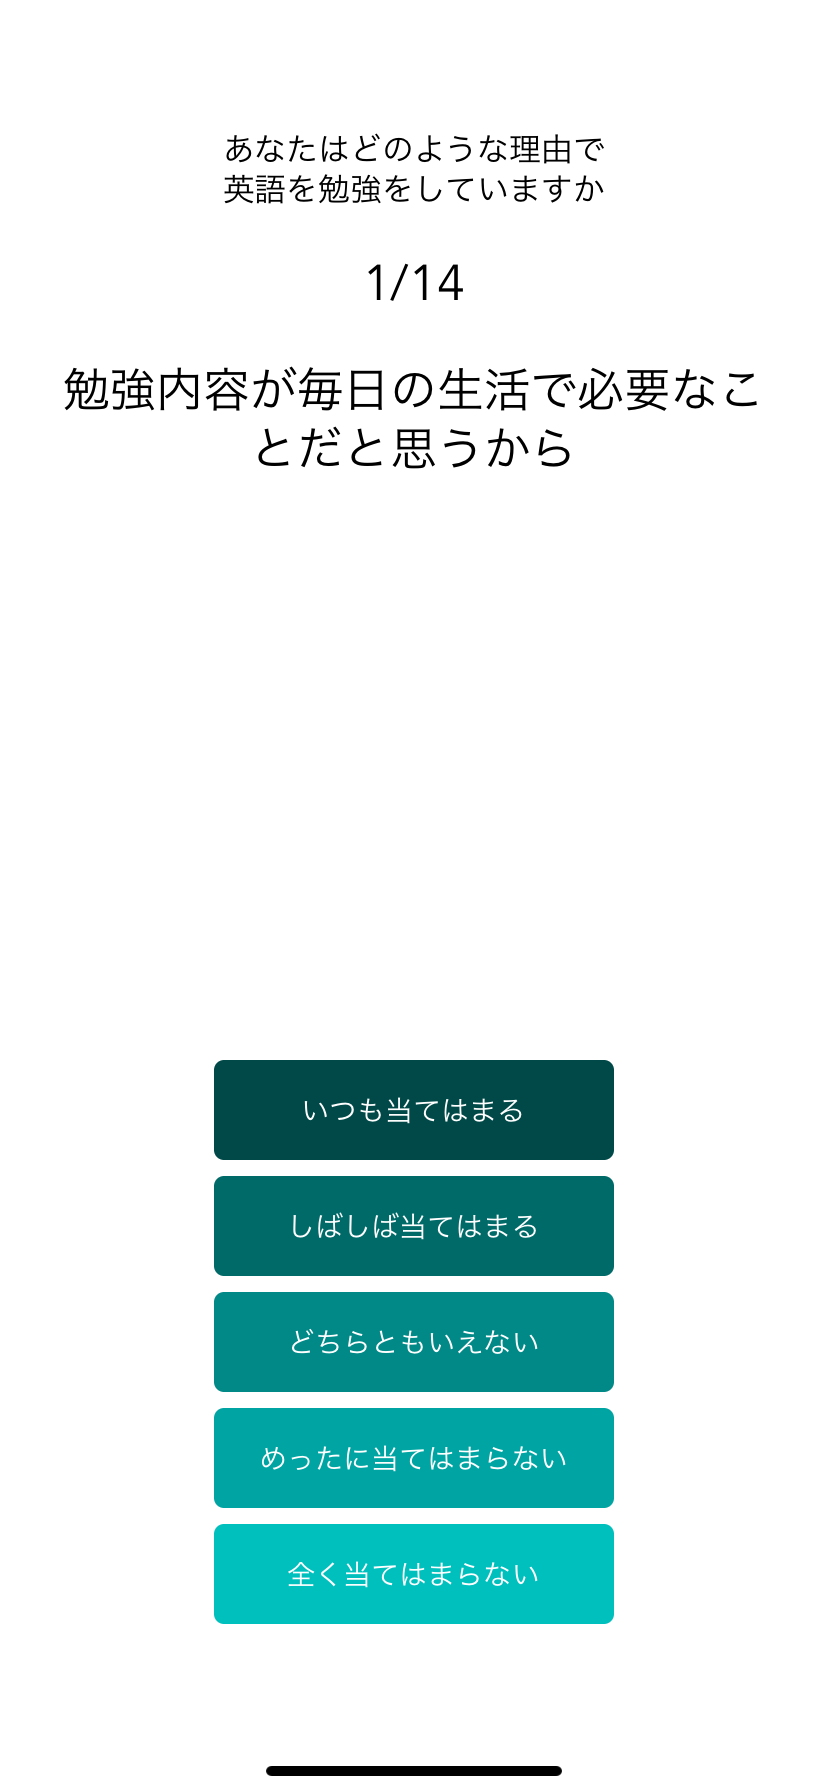
\includegraphics[width=5cm]{images/4/questionnaire.png}}
		\caption{アンケート回答画面}
		\label{fig:questionnaire4}
	\end{center}
	\end{minipage}

\end{tabular}
\end{center}
\end{figure}


\section{まとめ}
本章では,学習に対する動機づけの内在化を目的としたStuguinシステムを提案した.
また,Stuguinシステムの特徴および使用方法を述べた.
次章では,本システムの設計について述べる.